% Created by tikzDevice version 0.12.6 on 2026-07-03 11:54:54
% !TEX encoding = UTF-8 Unicode
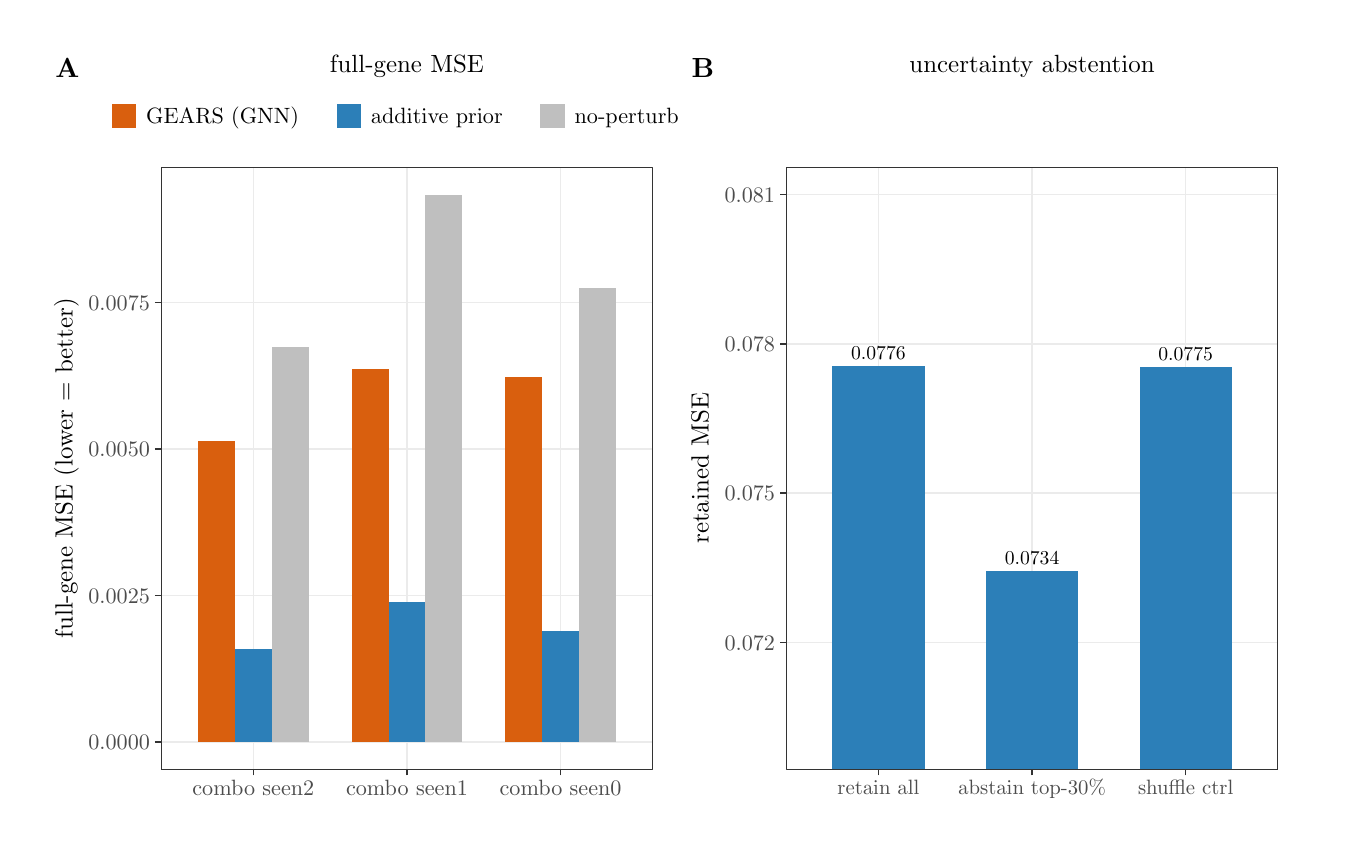
\begin{tikzpicture}[x=1pt,y=1pt]
\definecolor{fillColor}{RGB}{255,255,255}
\path[use as bounding box,fill=fillColor,fill opacity=0.00] (0,0) rectangle (469.75,289.08);
\begin{scope}
\path[clip] (  0.00,  0.00) rectangle (469.75,289.08);
\definecolor{drawColor}{RGB}{255,255,255}
\definecolor{fillColor}{RGB}{255,255,255}

\path[draw=drawColor,line width= 0.5pt,line join=round,line cap=round,fill=fillColor] (  0.00, -0.00) rectangle (469.75,289.08);
\end{scope}
\begin{scope}
\path[clip] (  5.00,  5.00) rectangle (234.88,284.08);
\definecolor{drawColor}{RGB}{255,255,255}
\definecolor{fillColor}{RGB}{255,255,255}

\path[draw=drawColor,line width= 0.5pt,line join=round,line cap=round,fill=fillColor] (  5.00,  5.00) rectangle (234.88,284.08);
\end{scope}
\begin{scope}
\path[clip] (234.88,  5.00) rectangle (460.75,284.08);
\definecolor{drawColor}{RGB}{255,255,255}
\definecolor{fillColor}{RGB}{255,255,255}

\path[draw=drawColor,line width= 0.5pt,line join=round,line cap=round,fill=fillColor] (234.88,  5.00) rectangle (460.75,284.08);
\end{scope}
\begin{scope}
\path[clip] ( 48.22, 21.12) rectangle (225.88,238.63);
\definecolor{fillColor}{RGB}{255,255,255}

\path[fill=fillColor] ( 48.22, 21.12) rectangle (225.88,238.63);
\definecolor{drawColor}{gray}{0.92}

\path[draw=drawColor,line width= 0.5pt,line join=round] ( 48.22, 31.00) --
	(225.88, 31.00);

\path[draw=drawColor,line width= 0.5pt,line join=round] ( 48.22, 83.93) --
	(225.88, 83.93);

\path[draw=drawColor,line width= 0.5pt,line join=round] ( 48.22,136.86) --
	(225.88,136.86);

\path[draw=drawColor,line width= 0.5pt,line join=round] ( 48.22,189.79) --
	(225.88,189.79);

\path[draw=drawColor,line width= 0.5pt,line join=round] ( 81.53, 21.12) --
	( 81.53,238.63);

\path[draw=drawColor,line width= 0.5pt,line join=round] (137.05, 21.12) --
	(137.05,238.63);

\path[draw=drawColor,line width= 0.5pt,line join=round] (192.57, 21.12) --
	(192.57,238.63);
\definecolor{fillColor}{RGB}{217,95,14}

\path[fill=fillColor] ( 61.55, 31.00) rectangle ( 74.87,139.82);
\definecolor{fillColor}{RGB}{44,127,184}

\path[fill=fillColor] ( 74.87, 31.00) rectangle ( 88.19, 64.67);
\definecolor{fillColor}{gray}{0.75}

\path[fill=fillColor] ( 88.19, 31.00) rectangle (101.52,173.70);
\definecolor{fillColor}{RGB}{217,95,14}

\path[fill=fillColor] (117.06, 31.00) rectangle (130.39,165.65);
\definecolor{fillColor}{RGB}{44,127,184}

\path[fill=fillColor] (130.39, 31.00) rectangle (143.71, 81.60);
\definecolor{fillColor}{gray}{0.75}

\path[fill=fillColor] (143.71, 31.00) rectangle (157.04,228.74);
\definecolor{fillColor}{RGB}{217,95,14}

\path[fill=fillColor] (172.58, 31.00) rectangle (185.91,162.90);
\definecolor{fillColor}{RGB}{44,127,184}

\path[fill=fillColor] (185.91, 31.00) rectangle (199.23, 71.23);
\definecolor{fillColor}{gray}{0.75}

\path[fill=fillColor] (199.23, 31.00) rectangle (212.55,194.87);
\definecolor{drawColor}{gray}{0.20}

\path[draw=drawColor,line width= 0.5pt,line join=round,line cap=round] ( 48.22, 21.12) rectangle (225.88,238.63);
\end{scope}
\begin{scope}
\path[clip] (  0.00,  0.00) rectangle (469.75,289.08);
\definecolor{drawColor}{gray}{0.30}

\node[text=drawColor,anchor=base east,inner sep=0pt, outer sep=0pt, scale=  0.80] at ( 44.17, 28.25) {0.0000};

\node[text=drawColor,anchor=base east,inner sep=0pt, outer sep=0pt, scale=  0.80] at ( 44.17, 81.18) {0.0025};

\node[text=drawColor,anchor=base east,inner sep=0pt, outer sep=0pt, scale=  0.80] at ( 44.17,134.10) {0.0050};

\node[text=drawColor,anchor=base east,inner sep=0pt, outer sep=0pt, scale=  0.80] at ( 44.17,187.03) {0.0075};
\end{scope}
\begin{scope}
\path[clip] (  0.00,  0.00) rectangle (469.75,289.08);
\definecolor{drawColor}{gray}{0.20}

\path[draw=drawColor,line width= 0.5pt,line join=round] ( 45.97, 31.00) --
	( 48.22, 31.00);

\path[draw=drawColor,line width= 0.5pt,line join=round] ( 45.97, 83.93) --
	( 48.22, 83.93);

\path[draw=drawColor,line width= 0.5pt,line join=round] ( 45.97,136.86) --
	( 48.22,136.86);

\path[draw=drawColor,line width= 0.5pt,line join=round] ( 45.97,189.79) --
	( 48.22,189.79);
\end{scope}
\begin{scope}
\path[clip] (  0.00,  0.00) rectangle (469.75,289.08);
\definecolor{drawColor}{gray}{0.20}

\path[draw=drawColor,line width= 0.5pt,line join=round] ( 81.53, 18.87) --
	( 81.53, 21.12);

\path[draw=drawColor,line width= 0.5pt,line join=round] (137.05, 18.87) --
	(137.05, 21.12);

\path[draw=drawColor,line width= 0.5pt,line join=round] (192.57, 18.87) --
	(192.57, 21.12);
\end{scope}
\begin{scope}
\path[clip] (  0.00,  0.00) rectangle (469.75,289.08);
\definecolor{drawColor}{gray}{0.30}

\node[text=drawColor,anchor=base,inner sep=0pt, outer sep=0pt, scale=  0.80] at ( 81.53, 11.56) {combo seen2};

\node[text=drawColor,anchor=base,inner sep=0pt, outer sep=0pt, scale=  0.80] at (137.05, 11.56) {combo seen1};

\node[text=drawColor,anchor=base,inner sep=0pt, outer sep=0pt, scale=  0.80] at (192.57, 11.56) {combo seen0};
\end{scope}
\begin{scope}
\path[clip] (  0.00,  0.00) rectangle (469.75,289.08);
\definecolor{drawColor}{RGB}{0,0,0}

\node[text=drawColor,rotate= 90.00,anchor=base,inner sep=0pt, outer sep=0pt, scale=  0.90] at ( 16.20,129.87) {full-gene MSE (lower = better)};
\end{scope}
\begin{scope}
\path[clip] (  0.00,  0.00) rectangle (469.75,289.08);
\definecolor{fillColor}{RGB}{255,255,255}

\path[fill=fillColor] ( 25.34,247.63) rectangle (248.76,266.63);
\end{scope}
\begin{scope}
\path[clip] (  0.00,  0.00) rectangle (469.75,289.08);
\definecolor{fillColor}{RGB}{255,255,255}

\path[fill=fillColor] ( 29.84,252.13) rectangle ( 39.84,262.13);
\definecolor{fillColor}{RGB}{217,95,14}

\path[fill=fillColor] ( 30.42,252.71) rectangle ( 39.26,261.55);
\end{scope}
\begin{scope}
\path[clip] (  0.00,  0.00) rectangle (469.75,289.08);
\definecolor{fillColor}{RGB}{255,255,255}

\path[fill=fillColor] (111.06,252.13) rectangle (121.06,262.13);
\definecolor{fillColor}{RGB}{44,127,184}

\path[fill=fillColor] (111.64,252.71) rectangle (120.48,261.55);
\end{scope}
\begin{scope}
\path[clip] (  0.00,  0.00) rectangle (469.75,289.08);
\definecolor{fillColor}{RGB}{255,255,255}

\path[fill=fillColor] (184.66,252.13) rectangle (194.66,262.13);
\definecolor{fillColor}{gray}{0.75}

\path[fill=fillColor] (185.24,252.71) rectangle (194.08,261.55);
\end{scope}
\begin{scope}
\path[clip] (  0.00,  0.00) rectangle (469.75,289.08);
\definecolor{drawColor}{RGB}{0,0,0}

\node[text=drawColor,anchor=base west,inner sep=0pt, outer sep=0pt, scale=  0.80] at ( 42.84,254.37) {GEARS (GNN)};
\end{scope}
\begin{scope}
\path[clip] (  0.00,  0.00) rectangle (469.75,289.08);
\definecolor{drawColor}{RGB}{0,0,0}

\node[text=drawColor,anchor=base west,inner sep=0pt, outer sep=0pt, scale=  0.80] at (124.06,254.37) {additive prior};
\end{scope}
\begin{scope}
\path[clip] (  0.00,  0.00) rectangle (469.75,289.08);
\definecolor{drawColor}{RGB}{0,0,0}

\node[text=drawColor,anchor=base west,inner sep=0pt, outer sep=0pt, scale=  0.80] at (197.66,254.37) {no-perturb};
\end{scope}
\begin{scope}
\path[clip] (  0.00,  0.00) rectangle (469.75,289.08);
\definecolor{drawColor}{RGB}{0,0,0}

\node[text=drawColor,anchor=base,inner sep=0pt, outer sep=0pt, scale=  0.90] at (137.05,272.88) {full-gene MSE};
\end{scope}
\begin{scope}
\path[clip] (  0.00,  0.00) rectangle (469.75,289.08);
\definecolor{drawColor}{RGB}{0,0,0}

\node[text=drawColor,anchor=base,inner sep=0pt, outer sep=0pt, scale=  1.00] at ( 14.35,271.12) {\bfseries A};
\end{scope}
\begin{scope}
\path[clip] (274.10, 21.12) rectangle (451.75,238.63);
\definecolor{fillColor}{RGB}{255,255,255}

\path[fill=fillColor] (274.10, 21.12) rectangle (451.75,238.63);
\definecolor{drawColor}{gray}{0.92}

\path[draw=drawColor,line width= 0.5pt,line join=round] (274.10, 66.96) --
	(451.75, 66.96);

\path[draw=drawColor,line width= 0.5pt,line join=round] (274.10,120.89) --
	(451.75,120.89);

\path[draw=drawColor,line width= 0.5pt,line join=round] (274.10,174.81) --
	(451.75,174.81);

\path[draw=drawColor,line width= 0.5pt,line join=round] (274.10,228.74) --
	(451.75,228.74);

\path[draw=drawColor,line width= 0.5pt,line join=round] (307.41, 21.12) --
	(307.41,238.63);

\path[draw=drawColor,line width= 0.5pt,line join=round] (362.93, 21.12) --
	(362.93,238.63);

\path[draw=drawColor,line width= 0.5pt,line join=round] (418.44, 21.12) --
	(418.44,238.63);
\definecolor{fillColor}{RGB}{44,127,184}

\path[fill=fillColor] (290.75,-1227.34) rectangle (324.07,166.90);

\path[fill=fillColor] (346.27,-1227.34) rectangle (379.58, 92.66);

\path[fill=fillColor] (401.79,-1227.34) rectangle (435.10,166.37);
\definecolor{drawColor}{RGB}{0,0,0}

\node[text=drawColor,anchor=base,inner sep=0pt, outer sep=0pt, scale=  0.71] at (307.41,169.35) {0.0776};

\node[text=drawColor,anchor=base,inner sep=0pt, outer sep=0pt, scale=  0.71] at (362.93, 95.11) {0.0734};

\node[text=drawColor,anchor=base,inner sep=0pt, outer sep=0pt, scale=  0.71] at (418.44,168.82) {0.0775};
\definecolor{drawColor}{gray}{0.20}

\path[draw=drawColor,line width= 0.5pt,line join=round,line cap=round] (274.10, 21.12) rectangle (451.75,238.63);
\end{scope}
\begin{scope}
\path[clip] (  0.00,  0.00) rectangle (469.75,289.08);
\definecolor{drawColor}{gray}{0.30}

\node[text=drawColor,anchor=base east,inner sep=0pt, outer sep=0pt, scale=  0.80] at (270.05, 64.20) {0.072};

\node[text=drawColor,anchor=base east,inner sep=0pt, outer sep=0pt, scale=  0.80] at (270.05,118.13) {0.075};

\node[text=drawColor,anchor=base east,inner sep=0pt, outer sep=0pt, scale=  0.80] at (270.05,172.06) {0.078};

\node[text=drawColor,anchor=base east,inner sep=0pt, outer sep=0pt, scale=  0.80] at (270.05,225.99) {0.081};
\end{scope}
\begin{scope}
\path[clip] (  0.00,  0.00) rectangle (469.75,289.08);
\definecolor{drawColor}{gray}{0.20}

\path[draw=drawColor,line width= 0.5pt,line join=round] (271.85, 66.96) --
	(274.10, 66.96);

\path[draw=drawColor,line width= 0.5pt,line join=round] (271.85,120.89) --
	(274.10,120.89);

\path[draw=drawColor,line width= 0.5pt,line join=round] (271.85,174.81) --
	(274.10,174.81);

\path[draw=drawColor,line width= 0.5pt,line join=round] (271.85,228.74) --
	(274.10,228.74);
\end{scope}
\begin{scope}
\path[clip] (  0.00,  0.00) rectangle (469.75,289.08);
\definecolor{drawColor}{gray}{0.20}

\path[draw=drawColor,line width= 0.5pt,line join=round] (307.41, 18.87) --
	(307.41, 21.12);

\path[draw=drawColor,line width= 0.5pt,line join=round] (362.93, 18.87) --
	(362.93, 21.12);

\path[draw=drawColor,line width= 0.5pt,line join=round] (418.44, 18.87) --
	(418.44, 21.12);
\end{scope}
\begin{scope}
\path[clip] (  0.00,  0.00) rectangle (469.75,289.08);
\definecolor{drawColor}{gray}{0.30}

\node[text=drawColor,anchor=base,inner sep=0pt, outer sep=0pt, scale=  0.75] at (307.41, 11.90) {retain all};

\node[text=drawColor,anchor=base,inner sep=0pt, outer sep=0pt, scale=  0.75] at (362.93, 11.90) {abstain top-30\%};

\node[text=drawColor,anchor=base,inner sep=0pt, outer sep=0pt, scale=  0.75] at (418.44, 11.90) {shuffle ctrl};
\end{scope}
\begin{scope}
\path[clip] (  0.00,  0.00) rectangle (469.75,289.08);
\definecolor{drawColor}{RGB}{0,0,0}

\node[text=drawColor,rotate= 90.00,anchor=base,inner sep=0pt, outer sep=0pt, scale=  0.90] at (246.08,129.87) {retained MSE};
\end{scope}
\begin{scope}
\path[clip] (  0.00,  0.00) rectangle (469.75,289.08);
\definecolor{drawColor}{RGB}{0,0,0}

\node[text=drawColor,anchor=base,inner sep=0pt, outer sep=0pt, scale=  0.90] at (362.93,272.88) {uncertainty abstention};
\end{scope}
\begin{scope}
\path[clip] (  0.00,  0.00) rectangle (469.75,289.08);
\definecolor{drawColor}{RGB}{0,0,0}

\node[text=drawColor,anchor=base,inner sep=0pt, outer sep=0pt, scale=  1.00] at (243.97,271.12) {\bfseries B};
\end{scope}
\end{tikzpicture}
